\documentclass[border=6pt]{standalone}
% Shared preamble for web figures.  Each figure is a standalone .tex that
% \input's this file; scripts/make-figures.sh turns it into an SVG.
% Handouts pull the same file with \fig{Unit_X/<name>}.
\usepackage[T1]{fontenc}
\usepackage{helvet}
\renewcommand{\familydefault}{\sfdefault}
\renewcommand{\ttdefault}{pcr}  % Courier: a real Type 1 typewriter font
\usepackage{amsmath}
\usepackage{tikz}
\usetikzlibrary{arrows.meta,positioning,calc,shapes.symbols,shapes.geometric}

% Who makes the rules is the point of most diagrams in this book, so the
% colors mean the same thing everywhere: blue is a person, orange is the
% computer, green is an answer, pink is the human brain.
\definecolor{person}{HTML}{2C6FAE}
\definecolor{machine}{HTML}{D35400}
\definecolor{result}{HTML}{1E8449}
\definecolor{brainpink}{HTML}{C2185B}
\definecolor{ink}{HTML}{2C3E50}

\tikzset{
  doodle/.style={line width=1.5pt, line cap=round, line join=round, draw=ink},
  box/.style={draw, rounded corners=5pt, line width=1.1pt, align=center,
              inner sep=7pt, minimum height=1.0cm, font=\small},
  personbox/.style={box, draw=person, fill=person!10},
  machinebox/.style={box, draw=machine, fill=machine!10},
  resultbox/.style={box, draw=result, fill=result!10},
  plainbox/.style={box, draw=ink!70, fill=ink!4},
  flow/.style={-{Stealth[length=8pt]}, line width=1.4pt, draw=ink},
}

% A person (blue) and a robot head (orange) as small icons.
% \personicon{x}{y}{scale}   \roboticon{x}{y}{scale}
\newcommand{\personicon}[3]{%
  \begin{scope}[shift={(#1,#2)}, scale=#3]
    \fill[person] (0,0.62) circle (0.28);
    \fill[person, rounded corners=6pt] (-0.42,-0.55) rectangle (0.42,0.28);
  \end{scope}}
\newcommand{\roboticon}[3]{%
  \begin{scope}[shift={(#1,#2)}, scale=#3]
    \draw[machine, line width=1.2pt] (0,0.5) -- (0,0.72);
    \fill[machine] (0,0.78) circle (0.08);
    \draw[machine, line width=1.4pt, fill=machine!12, rounded corners=4pt] (-0.5,-0.45) rectangle (0.5,0.5);
    \fill[ink] (-0.2,0.12) circle (0.08);
    \fill[ink] (0.2,0.12) circle (0.08);
    \draw[ink, line width=1pt] (-0.22,-0.22) -- (0.22,-0.22);
  \end{scope}}

\begin{document}
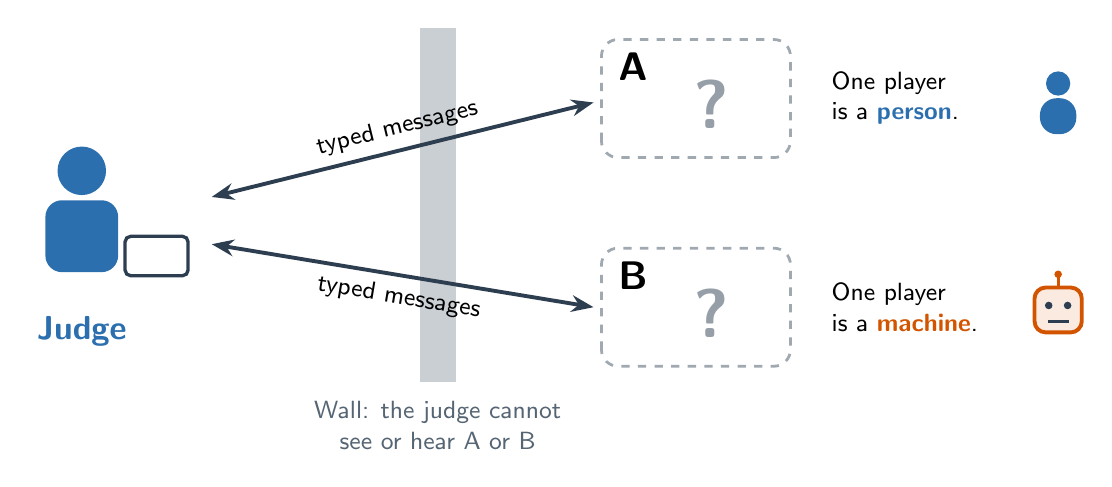
\begin{tikzpicture}
% Turing's imitation game: a judge sends text questions over a wall to two
% hidden players, A and B.  One is a person, one is a machine.

% judge
\personicon{0}{0.1}{1.1}
\draw[ink, line width=1.2pt, fill=white, rounded corners=2pt] (0.55,-0.55) rectangle (1.35,-0.05);
\node[font=\large\bfseries, text=person] at (0,-1.25) {Judge};

% wall
\fill[ink!25] (4.3,-1.9) rectangle (4.75,2.6);
\node[font=\small, text=ink!80, align=center] at (4.52,-2.45) {Wall: the judge cannot\\see or hear A or B};

% hidden players
\draw[ink!45, line width=1pt, dashed, rounded corners=6pt] (6.6,0.95) rectangle (9.0,2.45);
\node[font=\Large\bfseries] at (7.0,2.1) {A};
\node[font=\fontsize{30}{30}\selectfont\bfseries, text=ink!50] at (8.0,1.62) {?};
\draw[ink!45, line width=1pt, dashed, rounded corners=6pt] (6.6,-1.7) rectangle (9.0,-0.2);
\node[font=\Large\bfseries] at (7.0,-0.55) {B};
\node[font=\fontsize{30}{30}\selectfont\bfseries, text=ink!50] at (8.0,-1.03) {?};

% messages: typed text only, both ways
\draw[{Stealth[length=8pt]}-{Stealth[length=8pt]}, line width=1.4pt, draw=ink] (1.65,0.45) -- node[above, sloped, font=\small] {typed messages} (6.5,1.65);
\draw[{Stealth[length=8pt]}-{Stealth[length=8pt]}, line width=1.4pt, draw=ink] (1.65,-0.15) -- node[below, sloped, font=\small] {typed messages} (6.5,-0.95);

% key
\node[anchor=west, align=left, font=\small] at (9.4,1.7) {One player\\is a \textbf{\textcolor{person}{person}}.};
\personicon{12.4}{1.55}{0.55}
\node[anchor=west, align=left, font=\small] at (9.4,-0.95) {One player\\is a \textbf{\textcolor{machine}{machine}}.};
\roboticon{12.4}{-1.0}{0.6}
\end{tikzpicture}
\end{document}
